\documentclass{scrartcl}
\usepackage{amsmath,amssymb,commath,graphicx,enumerate,listings}
\setkomafont{disposition}{\normalfont\bfseries}

\title{Mat 354}
\subtitle{Homework 14}
\author{Kenny Roffo}
\date{Due November 23, 2015}

\begin{document}
\maketitle

\begin{enumerate}
  
\item A random variable with the Gamma distribution has mean 5. The scale and shape parameters are equal.

  \begin{enumerate}[a)]
  \item Accurately sketch the probability density function.

    For a gamma distribution, we know the mean is $E(Y) = \alpha\beta$. Since $\alpha=\beta$, this implies $\alpha=\beta=\sqrt{5}$.
    Thus the pdf for this distribution is $$f(y) = \begin{cases} \frac{y^{\sqrt{5}-1}e^{-y/\sqrt{5}}}{\Gamma(\sqrt{5})\sqrt{5}^{\sqrt{5}}} & y > 0 \\ 0 & y \le 0 \end{cases}$$ We can plot this in R using dgamma(y,shape=sqrt(5),scale=sqrt(5)).\\
    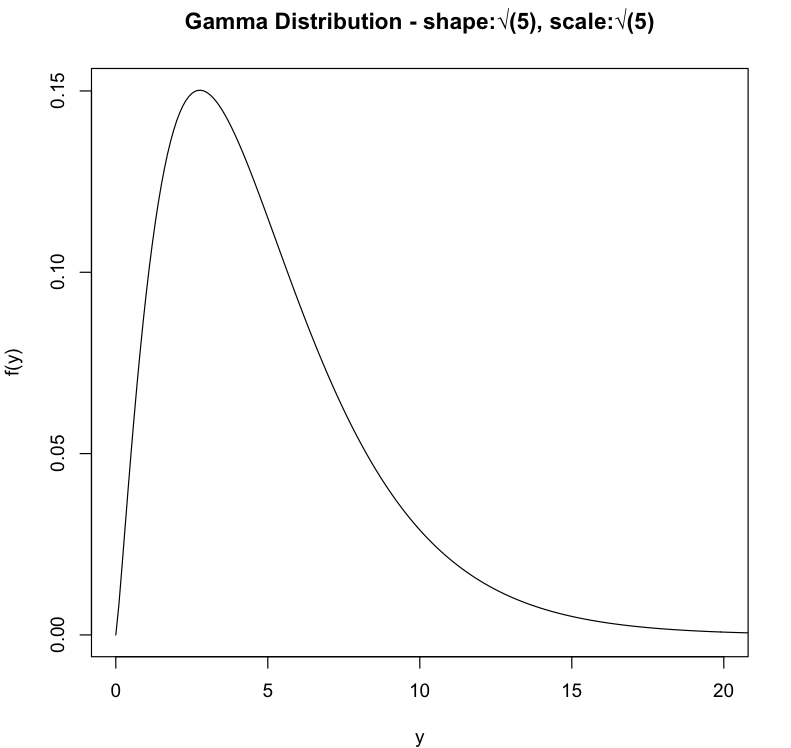
\includegraphics[keepaspectratio=true, scale=0.35]{1a.png}

  \item Find the probability of a result within 1 standard deviation of the mean.\\

    The standard deviation is $$\sigma = \sqrt{\sqrt{5}\sqrt{5}^2} = \sqrt{5\sqrt{5}}$$ Thus the probability of a result being within 1 standard deviation of the mean is found in R using \\pgamma(5+sqrt(5*sqrt(5)),shape=sqrt(5),scale=sqrt(5)) - \\pgamma(5-sqrt(5*sqrt(5)),shape=sqrt(5),scale=sqrt(5))

    The resulting probability is 0.7299\\

  \item Find the probability of a result within 2 standard deviations of the mean.\\

    To find this we simply plug the same command as before into R, but now we multiply the standard deviations by 2 before adding/subtracting from the mean. The result is 0.9540.\\

  \item Find the five number summary (OK – find 4/5ths of the five number summary, as technically there is no maximum).\\

    We know the minimum is 0, so we just need to find the quartiles using qgamma in R. Doing so, we obtain 4/5ths of the five number summary: $$\{0,2.5418,4.2776,6.6983,\text{DNE}\}$$


  \end{enumerate}


\item (For right skewed distributions it is generally the case that Mode $<$ Median $<$ Mean. All Gamma distributions are right skewed.) A random variable has Gamma distribution with mean 10 and standard deviation 5. Find the mode and median. (Recall that the mode is the value $y$ with maximum density.) Explain how you arrive at your value for the mode.\\

  To find the median we can simply use qgamma. However, it is not quite that simple. We first need to find out what the shape and scale ($\alpha$ and $\beta$) are! We know the mean and standard deviation are $\mu = \alpha\beta = 10$ and $\sigma=\sqrt(\alpha)\beta = 5$ respectively. We just need to solve these equations for $\alpha$ and $\beta$:
  \begin{align*}
    &10 = \alpha\beta\\
    \implies&\frac{10}{\alpha} = \beta\\
    \implies&5 = \frac{10}{\sqrt{\alpha}}\\
    \implies& \alpha = \frac{100}{25} = 4\\
    \implies& \beta = \frac{10}{4} = 2.5
  \end{align*}

  And now we find the median to be qgamma(0.5,shape=4,scale=2.5) = 9.1802. As for the mode, we can do the following:
  \begin{lstlisting}[language=R]
    > y <- seq(0,200000)/10000
    > f <- dgamma(y,shape=4,scale=2.5)
    > y[max(f) = = f]
  \end{lstlisting}
  What is happening here is we are finding the maximum of the density at values from 0 to 20 counting up by 0.0001 each step. We are assuming the density's big ole hump has relaxed before the value 20, but that's a safe assumption here, considering it does. Also, this will only give us a value accurate to 4 decimal places, but that's precise enough for us. Anyway, the mode turns out to be 7.5.


  %% \item For the Gamma random variable $Y$ with $\alpha = 1⁄2$ and $\beta = 2$.

  %% \begin{enumerate}[a)]
  %% \item What is the expected value? The variance?\\

  %%   The expected value is $E(Y) = \alpha\beta = 1$ and the variance is $V(Y) = \alpha\beta^2 = 2$.

  %% \item Determine $P\left(Y\le\frac{9k^2}{25}\right)$ for $k \in [1,6] \cap \mathbb{Z}$\\
  %%   These values are easily computed using R:
  %%   \begin{lstlisting}[language=R]
  %%   > k <- seq(1,6)
  %%   > pgamma((3*k/5)^2,shape=1/2,scale=2)
  %% \end{lstlisting}
  %%   We find the probabilities are:

  %%   $k=1$: 0.4514938\\

  %%   $k=2$: 0.7698607\\

  %%   $k=3$: 0.9281394\\

  %%   $k=4$: 0.9836049\\

  %%   $k=5$: 0.9973002\\

  %%   $k=6$: 0.9996818\\
  
  %% \end{enumerate}


  %% \item For a Normal random variable:

  %% \begin{enumerate}[a)]
  %% \item Determine as accurately as possible the probability of a result within $3k/5$ standard deviations of the mean, for $k \in [1,6] \cap \mathbb{Z}$.\\


  %% Determine $E(Z^2)$ where $Z$ denotes the Standard Normal random variable.


  %% \end{enumerate}


  %% \item Suggest a relationship between the variables $X$ of problem 3 and $Z$ of problem 4. Based on that relationship conjecture as to the value of $E(Z^4)$\\


\item (Really problem 6) Survival times are distributed according to the Gamma distribution with shape and scale parameters both equal to 2.

  \begin{enumerate}[a)]
  \item Determine the mean and standard deviation of survival times.\\
    The mean is $E(Y) = \alpha\beta = 4$ and the standard deviation is $\sigma = \sqrt{\alpha}\beta = 2\sqrt{2}$.

  \item Determine the probability a survival time is greater than 3.\\
    The probability a survival time is greater than 3 is
    \begin{align*}
      P(Y > 3) &= 1 - P(Y \le 3)\\
      &= 1 - \text{pgamma(3,shape=2,scale=2)}\\
      &= 0.5578
    \end{align*}

    Five values are randomly and independently sampled from this distribution. Consider the random variable $L$, the minimum survival time for the sample of five values.

  \item Determine the probability the minimum survival time exceeds 3.\\
    
    First we note the distribution function of $L$ is $$P(L \le l) = P(Y \ge l)^5 = \left(1 - P(Y \le l)\right)^5$$ Now we see 
    \begin{align*}
      P(L > 3) &= 1 - P(L \le 3)\\
      &= 1 - \left(1 - P(Y \le 3)\right)^5\\
      &= 1 - \left(1 - \text{pgamma(3,shape=2,scale=2)}\right)^5\\
      &= 0.9460
    \end{align*}
    
    Parts d and e Extra. I thought about this for a few seconds, but it's not obvious to me how to do them.
  \item If $g(l)$ is the density function for the minimum, what is the value of $g(3)$?\\\ \\\ \\\ \\
    

  \item Determine the expected value and variance of $L$.
  \end{enumerate}
\end{enumerate}
\end{document}

